\section{Recognition system}

%	ake classy tam budu (samostatny dataset, trainer, tester)
% potom opiseme nejaku strukturu siete
% ze ju programuje v pytorchi a mozno povedat ze aku verziu cudy a nejake packages
% mozno class diagram 
% programovacie prostredie python, pytorch, verzia cudy
% parametre mojho pocitaca na ktory to deploynem


%outline:
%uvod
%    - ze je to skript v pythone
%    - ze pouzivam nejake packages zname
%    - ze je to deploynute tam a tam
%project structure
%    - kazdu triedu opisat 
%    - class diagram
%    - deklaraciu CNN

The system is implemented in Python in a form of Jupyter notebook. The network is implemented using Pytorch library with Cuda 11.3. Other useful packages include: numpy, scipy, matplotlib, sklearn, astropy, etc. 


\subsection{Deployment}
The training of the network is running on the desktop computer with Microsoft Windows 10 Pro operating system. The hardware consists of the following:
\begin{itemize}
    \item Intel(R) Core(TM) i7-6700 CPU @ 3.40GHz, 3401 MHz, with 4 cores and 8 logical processors 
    \item NVIDIA GeForce GTX 1050 Ti
    \item 16GB of RAM memory
\end{itemize}

\subsection{Project structure}

As mentioned before the system is written in the Jupyter notebook. This allows us to train multiple times, without having to load the data every time. It is also easier to configure the parameters of the network and see the progress in real-time. 

The structure of the notebook is divided into multiple cells to allow us to run the specific cell we need without having to run redundant operations. To improve the quality of the script we have created multiple helpful classes, depicted in the Figure \ref{img:networkClass}: 

\begin{itemize}
    \item \textbf{MyDataLoader} \\
    The class loads all training, validation, and testing data from folders and parses them into the Dataset class. It uses the name of the folders to assign labels to each image.
    
    \item \textbf{FITSDataset} \\
    The class implements torch.utils.data.Dataset class and loads FITS images into tensors. It also provides an option to pre-process data before loading them into tensors. 
    
    \item \textbf{DataAugmentation} \\
    Implements data augmentation techniques explained in the Section \ref{sec:parametersNetwork}. 
    
    \item \textbf{MyCNN} \\
    Contains a declaration of each layer of the convolutional neural network. Implements torch.nn.Module class. 
    
    \item \textbf{EarlyStopping} \\
    Performs the early stopping technique described in the Section \ref{sec:parametersNetwork}. 
    
    \item \textbf{Visualizer} \\
    Plots the evolution of loss and accuracy during training. The plotted images are saved as JPEG files in the defined destination folder. 
    
    \item \textbf{Trainer} \\
    The class implements the training and validation of the network. It contains methods for forward and backward pass of the network. It stores the training and validation loss and observes its progress for the early stopping algorithm. 
    
    \item \textbf{Tester} \\
    Evaluates the network using testing data. It outputs the accuracy, recall, and precision of the trained model as well as plots confusion matrices. Moreover, it saves images that were wrongly classified during evaluation. 
\end{itemize}

\begin{figure}[h]
    \centering
    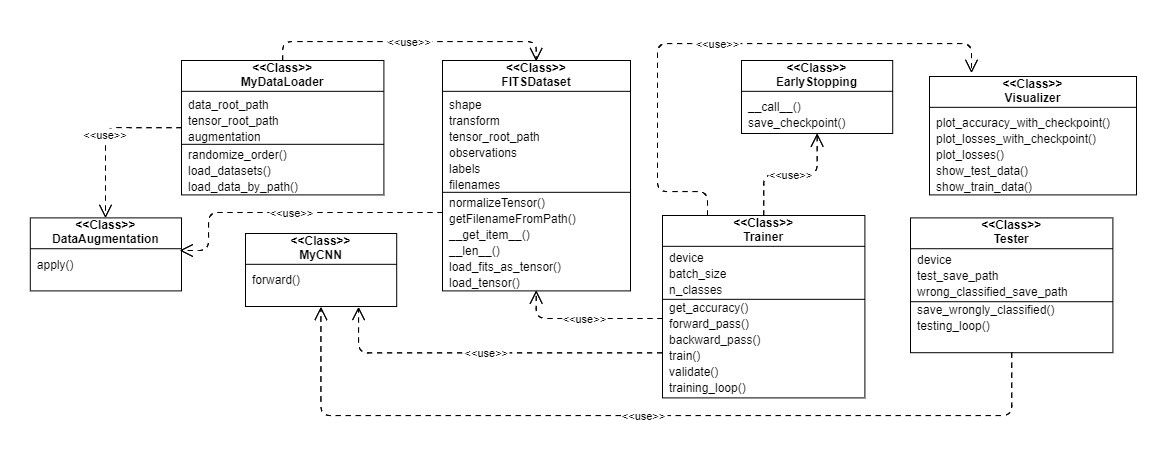
\includegraphics[width=\textwidth]{images/classDiagramNetwork.png}
    \caption{Class diagram of the recognition system.}
    \label{img:networkClass}
\end{figure}

